\section{Power Functions and Polynomial Functions}
In order to better understand the bird problem, we need to understand a specific type of function. A power function is a
function with a single term that is the product of a real number, a coefficient, and a variable raised to a fixed real
number. (A number that multiplies a variable raised to an exponent is known as a coefficient.)
As an example, consider functions for area or volume. The function for the area of a circle with radius $r$ is
$A(r) = \pi r^2$. The function for the volume of a sphere with radius $r$ is $V(r) = \frac{4}{3} \pi r^3$. These are both power
functions because they consist of a coefficient and a variable raised to a fixed power. 

In conclusion A power function is a function that can be represented in the form $$f(x)=kx^p$$ where $k$ and $p$ are real numbers, and $k$ is known as the coefficient.

\subsection{Identifying End Behaviour of Power Functions}
The figure shows the graphs of $f(x)=x^2$, $g(x)=x^4$ and $h(x)=x^6$ which are all power functions with even, wholenumber powers. Notice that these graphs have similar shapes, very much like that of the quadratic function in the
toolkit. However, as the power increases, the graphs flatten somewhat near the origin and become steeper away from
the origin.

\begin{align*}
    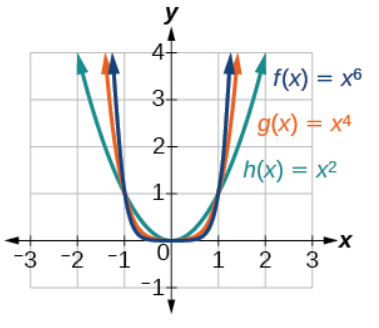
\includegraphics[width=1\textwidth]{algebra-pre-calculus/algebra/power-functions-and-polynomial-functions/even_power_functions.png}
\end{align*} \break

With the even-power function, as the input increases or decreases without bound, the output values become very large,
positive numbers. Equivalently, we could describe this behavior by saying that as $x$ approaches positive or negative
infinity, the $f(x)$ values increase without bound. In symbolic form, we could write

$$ x\rightarrow \pm \infty, f(x)\rightarrow \infty$$

\begin{align*}
    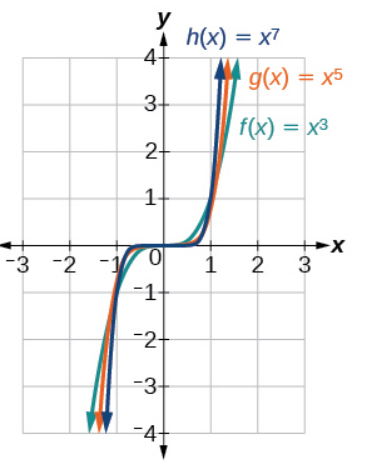
\includegraphics[width=1\textwidth]{algebra-pre-calculus/algebra/power-functions-and-polynomial-functions/odd_power_functions.png}
\end{align*} \break

$$ x\rightarrow - \infty, f(x)\rightarrow - \infty $$
$$ x\rightarrow \infty, f(x)\rightarrow \infty $$

The behavior of the graph of a function as the input values get very small ( $x\rightarrow-\infty$ ) and get very large ( $x\rightarrow \infty$ ) is
referred to as the end behavior of the function. We can use words or symbols to describe end behaviour.

\begin{align*}
    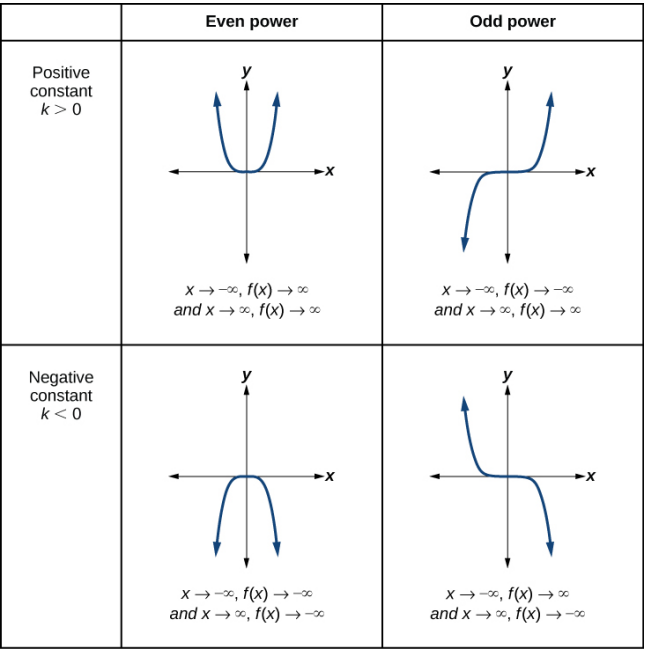
\includegraphics[width=1\textwidth]{algebra-pre-calculus/algebra/power-functions-and-polynomial-functions/even_odd_power.png}
\end{align*} \break

\subsection{Identifying Polynomial Functions}
A polynomial function consists of either zero or the sum of a finite
number of non-zero terms, each of which is a product of a number, called the coefficient of the term, and a variable
raised to a non-negative integer power.

\begin{align*}
    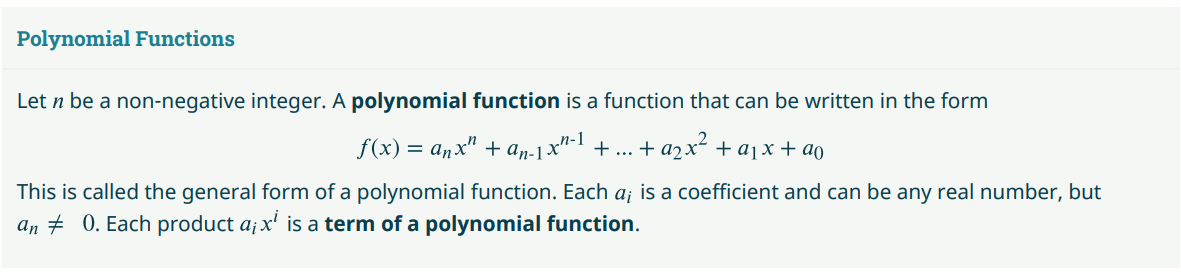
\includegraphics[width=1.4\textwidth]{algebra-pre-calculus/algebra/power-functions-and-polynomial-functions/polynomial_function_identifiy.png}
\end{align*} \break

\subsection{Identifying the Degree and Leading Coefficient of a Polynomial Function}
Because of the form of a polynomial function, we can see an infinite variety in the number of terms and the power of the
variable. Although the order of the terms in the polynomial function is not important for performing operations, we
typically arrange the terms in descending order of power, or in general form. The degree of the polynomial is the
highest power of the variable that occurs in the polynomial; it is the power of the first variable if the function is in
general form. The leading term is the term containing the highest power of the variable, or the term with the highest
degree. The leading coefficient is the coefficient of the leading term.

\begin{align*}
    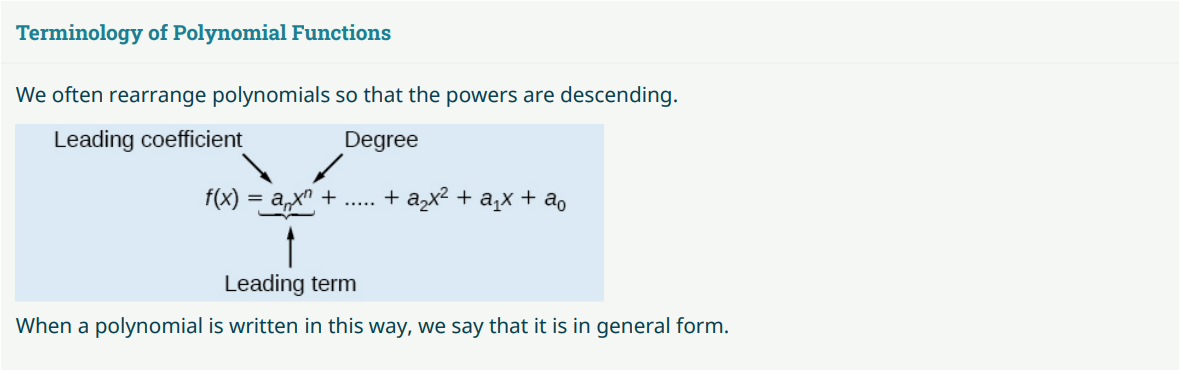
\includegraphics[width=1.4\textwidth]{algebra-pre-calculus/algebra/power-functions-and-polynomial-functions/leading_coefficient.png}
\end{align*} \break

For example $f(x)=3x^2+2x-1$ is a polynomial function in general form. The degree of the polynomial is 2, the leading term is $3x^2$, and the leading coefficient is 3.

\subsection{Identifying the End Behavior of Polynomial Functions}

Knowing the degree of a polynomial function is useful in helping us predict its end behavior. To determine its end
behavior, look at the leading term of the polynomial function. Because the power of the leading term is the highest, that
term will grow significantly faster than the other terms as $x$ gets very large or very small, so its behavior will dominate
the graph. For any polynomial, the end behavior of the polynomial will match the end behavior of the term of highest
degree. See these figures below.

\begin{align*}
    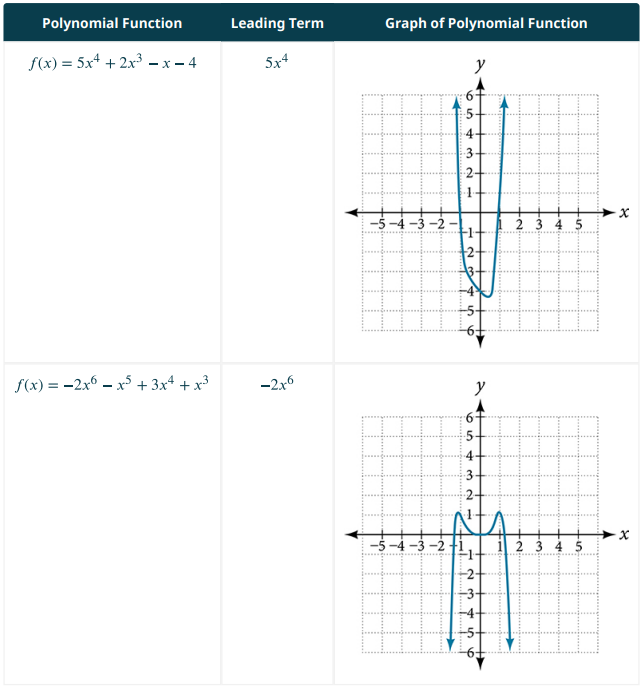
\includegraphics[width=1\textwidth]{algebra-pre-calculus/algebra/power-functions-and-polynomial-functions/pol_table1.png}\\
    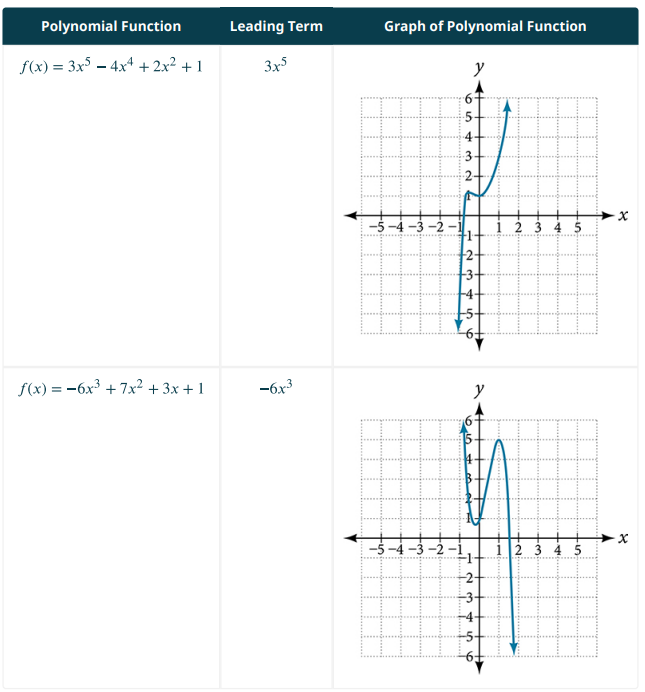
\includegraphics[width=1\textwidth]{algebra-pre-calculus/algebra/power-functions-and-polynomial-functions/pol_table2.png}
\end{align*} \break

For further information check out this \url{https://www.khanacademy.org/math/algebra2/x2ec2f6f830c9fb89:poly-graphs/x2ec2f6f830c9fb89:poly-end-behavior/a/end-behavior-of-polynomials}

